\begin{figure}[h!]
\centering
    \begin{tikzpicture}[scale=1]
\draw[step=0.5cm,color=gray] (0.0,0.0) grid (2,1);
\node at (0.75,0.75) {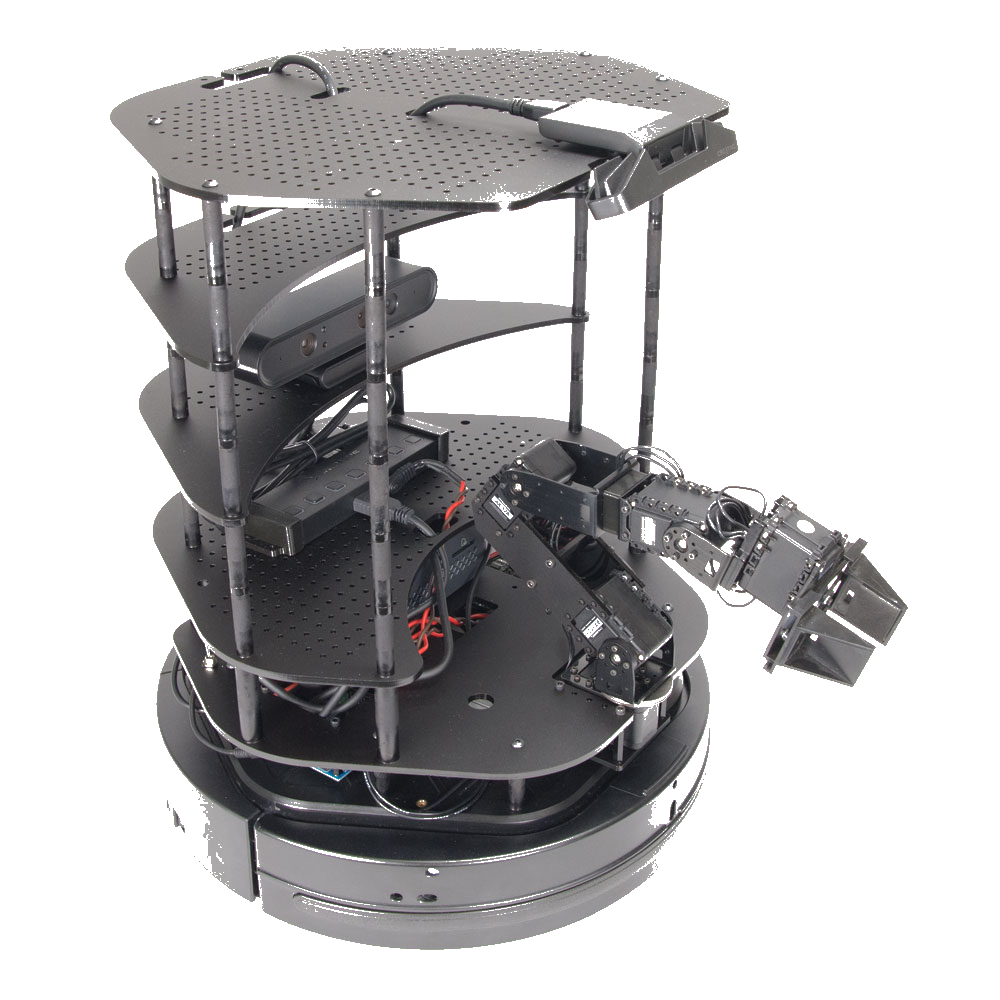
\includegraphics[scale=0.015]{figs/agent.png}};
\node at (-1.25,0.75)
{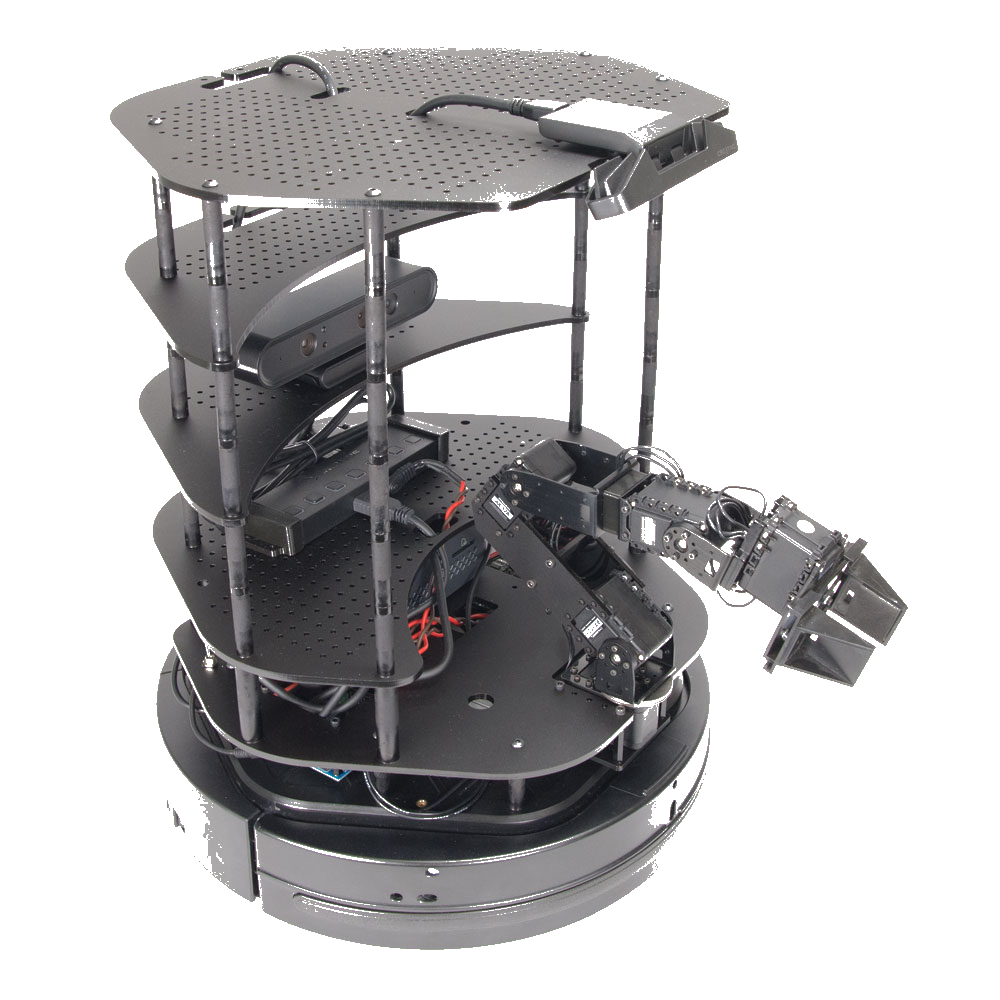
\includegraphics[scale=0.015]{figs/agent.png}};

\filldraw[fill=red!80!white,draw=black] (-0.5,1.0) rectangle (-1.0,0.5);
\filldraw[fill=red!80!white,draw=black] (-0.5,0.5) rectangle (-1.0,-0);

\filldraw[fill=red!80!white,draw=black] (-0.5,-0.5) rectangle (-1.0,-1.0);
\filldraw[fill=red!80!white,draw=black] (-0.5,-1.0) rectangle (-1.0,-1.5);

\filldraw[fill=red!80!white,draw=black] (-0.5,-2.0) rectangle (-1.0,-2.5);
\filldraw[fill=red!80!white,draw=black] (-0.5,-2.5) rectangle (-1.0,-3.0);

\filldraw[fill=orange!30!white,draw=black] (1.0,-0.5) rectangle (0.5,-1.0);
\filldraw[fill=blue!30!white,draw=black] (-2.5,-0.5) rectangle (-2.0,-1.0);

\end{tikzpicture}

    \caption{Gridworld with 2 agents needing to reach respective goals}
    \label{fig:exp2}
\end{figure}
